\documentclass[11pt]{article}

%defines page size and margins
\usepackage{geometry}
\geometry{
  letterpaper,
  left=1in,
  right=1in,
  top=1in,
  bottom=1in,
}

%Sets spacing for entire document
\usepackage{setspace}
\singlespacing

%Package for reducing space in between list items
\usepackage{enumitem}

%Links
\usepackage{hyperref}

%Math symbols
\usepackage{gensymb}

%For floating images
\usepackage{float}

%better tables
\usepackage{multirow}
\usepackage{array}

\usepackage{longtable}

%Used for adjusting images
\usepackage[export]{adjustbox}

%Image path
\usepackage{graphicx}
\usepackage{animate}

\begin{document}

{\Large\noindent Brett Levenson, Andy Poulos, Rishabh Shah, John Stefan

\noindent September 19, 2017

\noindent Lab 1 \\}

\noindent\textbf{Exercise One:}

\noindent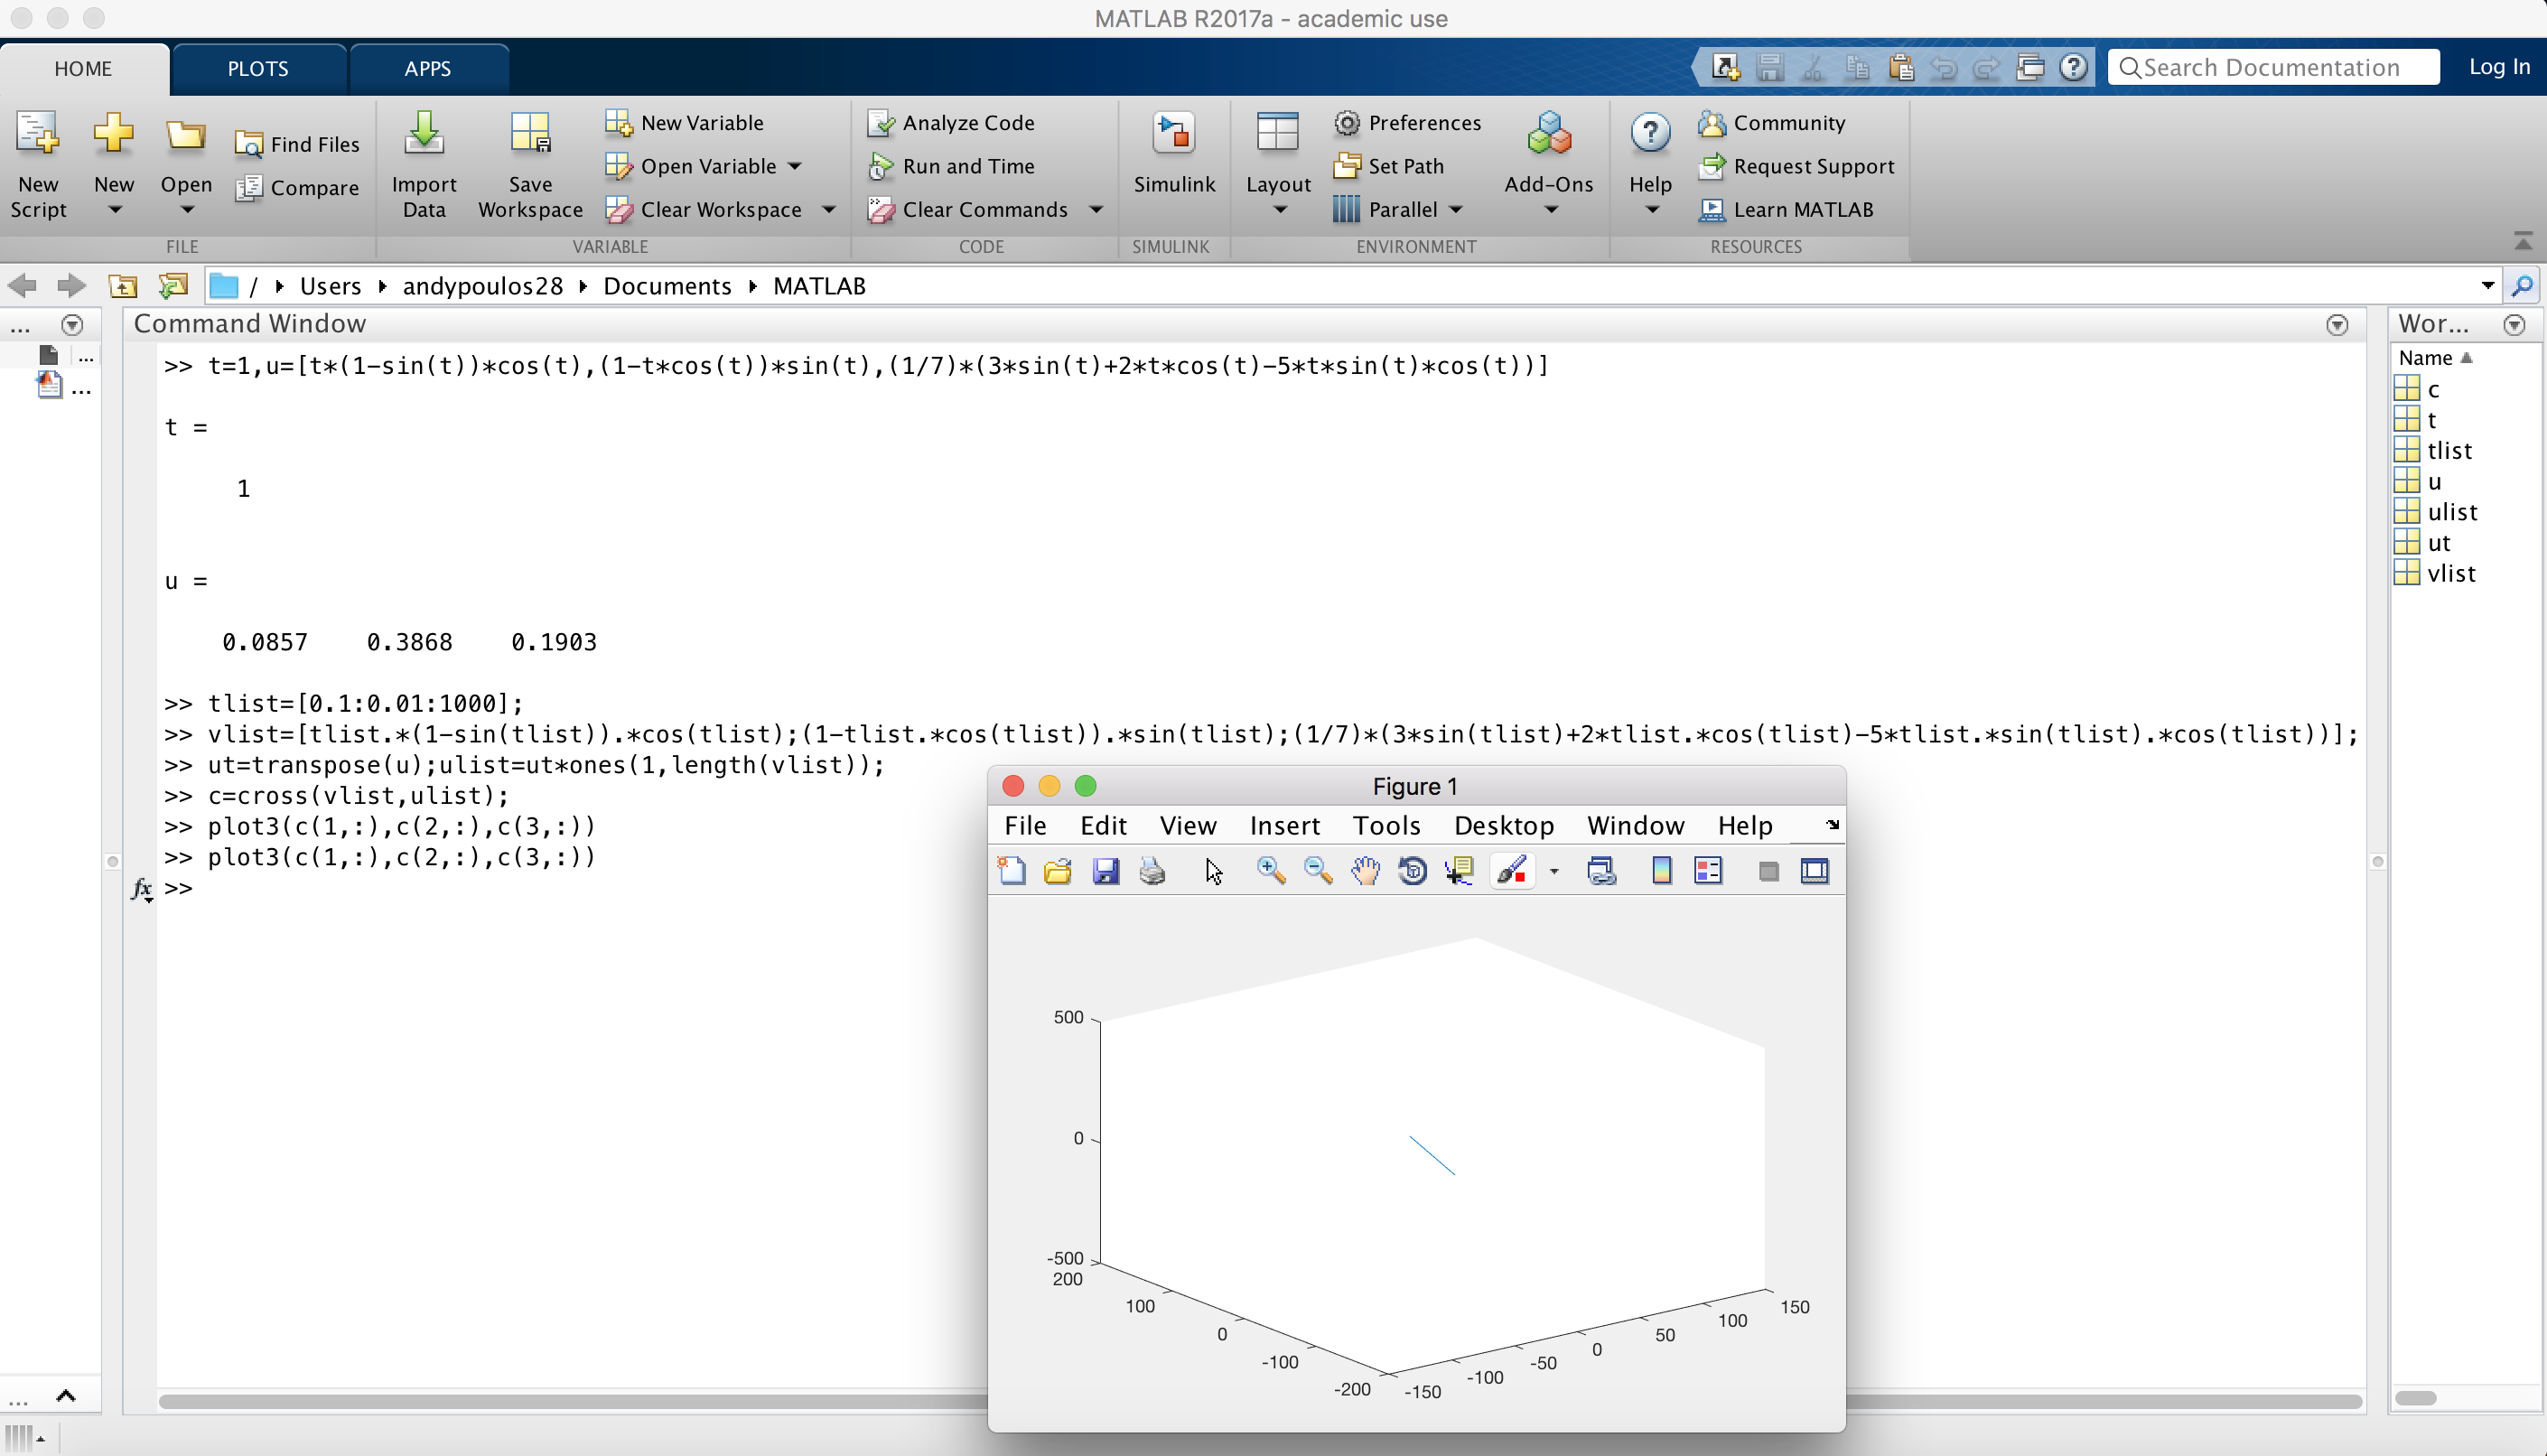
\includegraphics[scale=0.3]{One} \\

\noindent\textbf{Exercise Two:}

\begin{figure}[H]
	\caption{The trend is for the data to increase linearly.}
	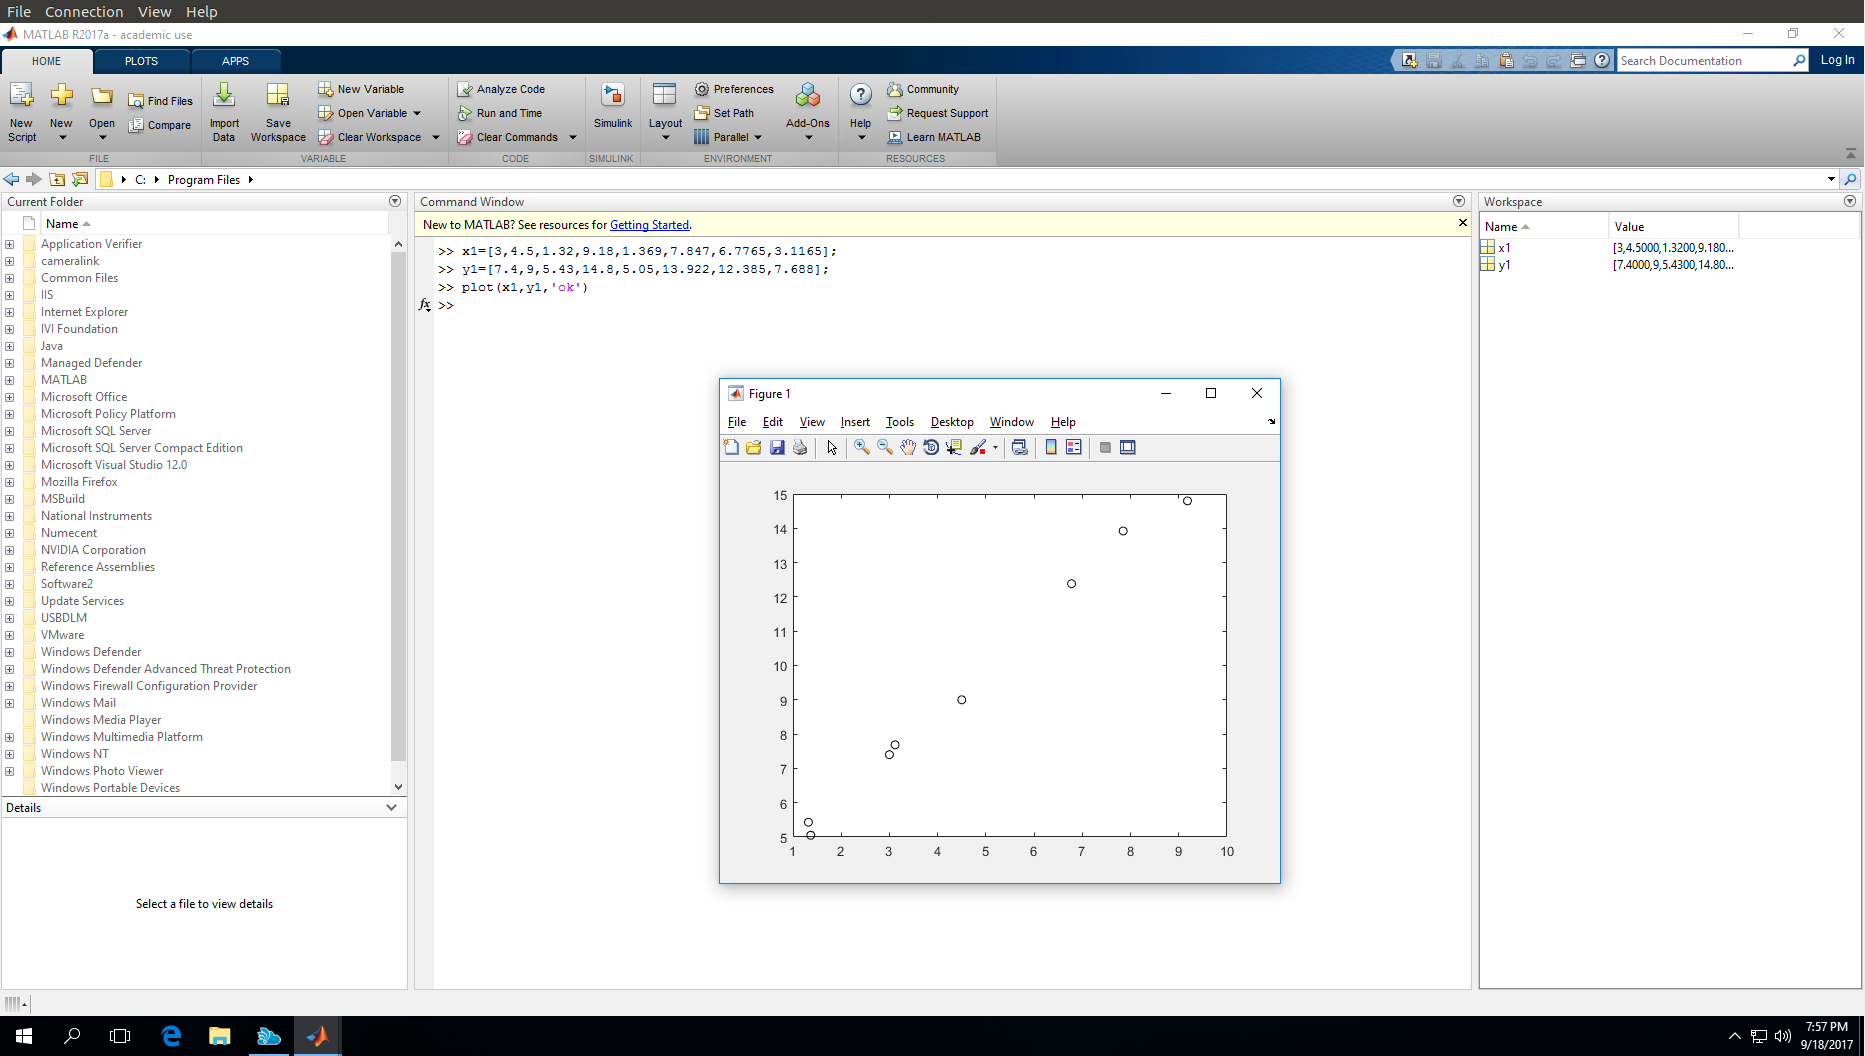
\includegraphics[scale=0.25]{Two}
\end{figure}

\newpage

\noindent\textbf{Exercise Three:}

\noindent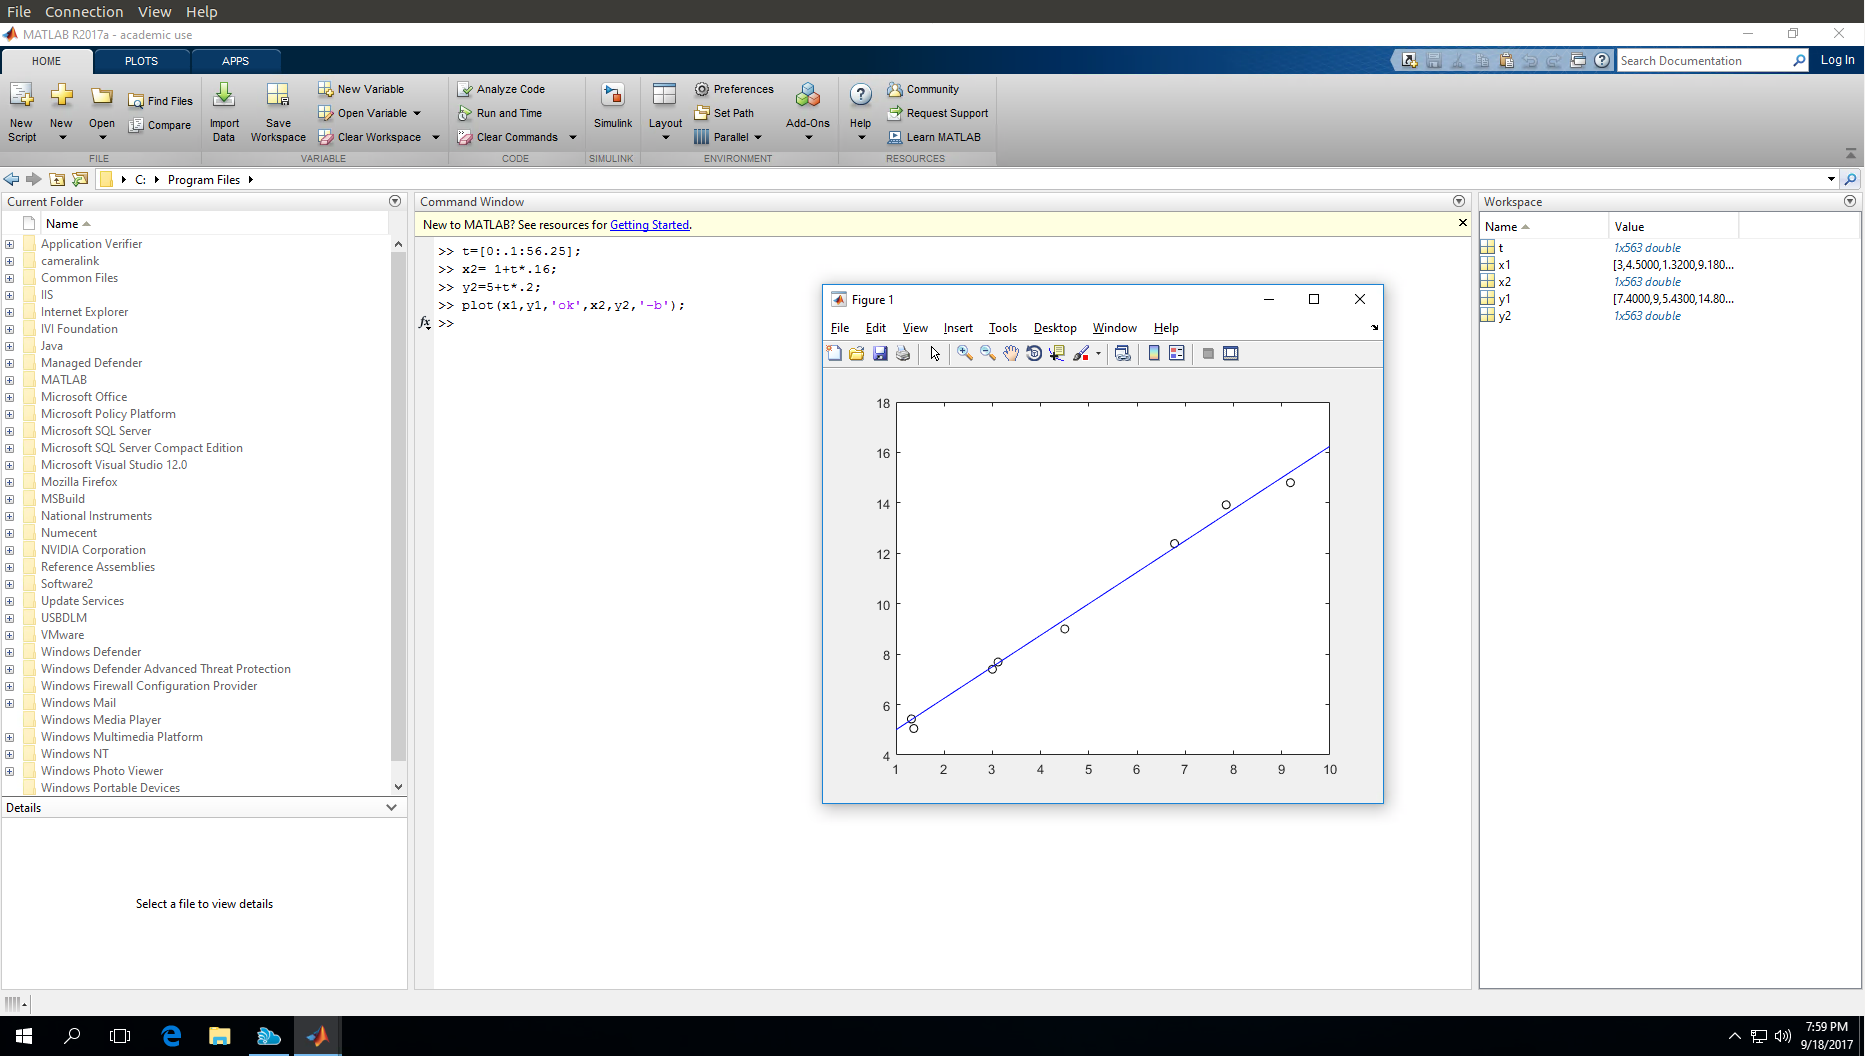
\includegraphics[scale=0.25]{Three} \\

\noindent\textbf{Exercise Four:}

\noindent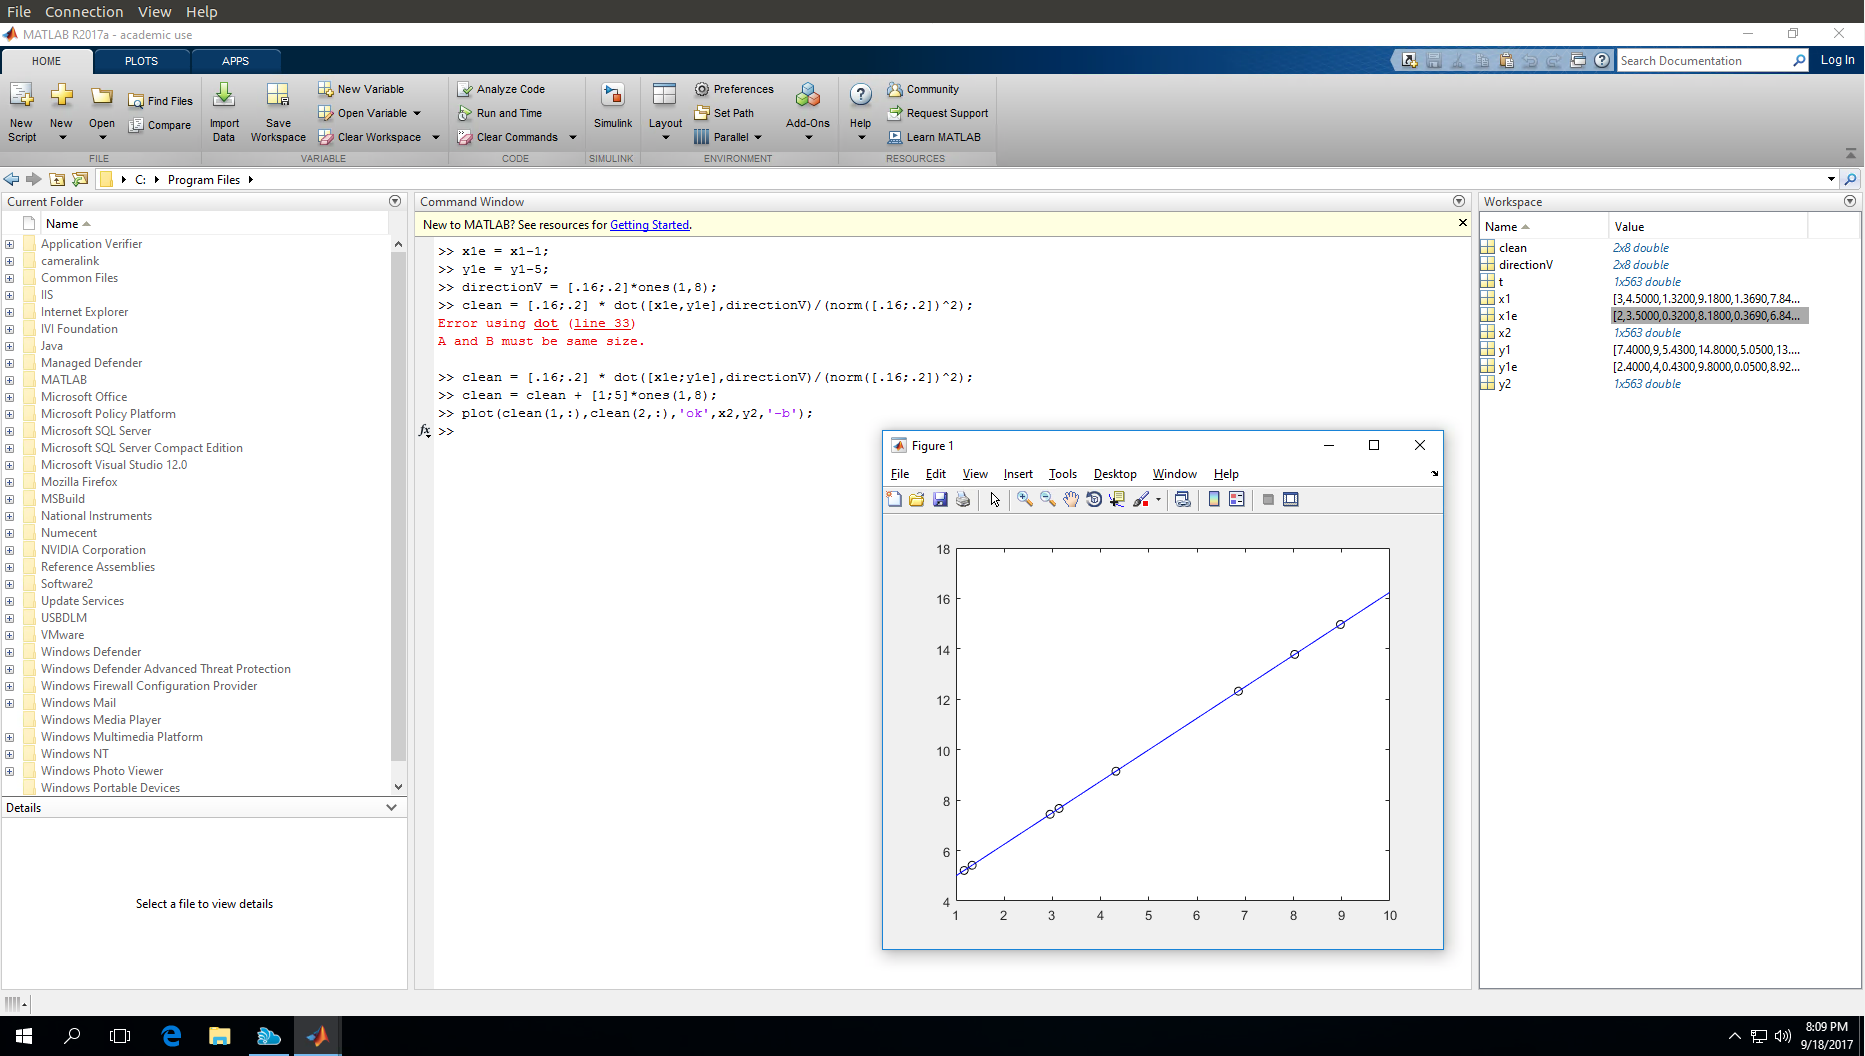
\includegraphics[scale=0.25]{Four} \\

\newpage

\noindent\textbf{Exercise Five:}

\noindent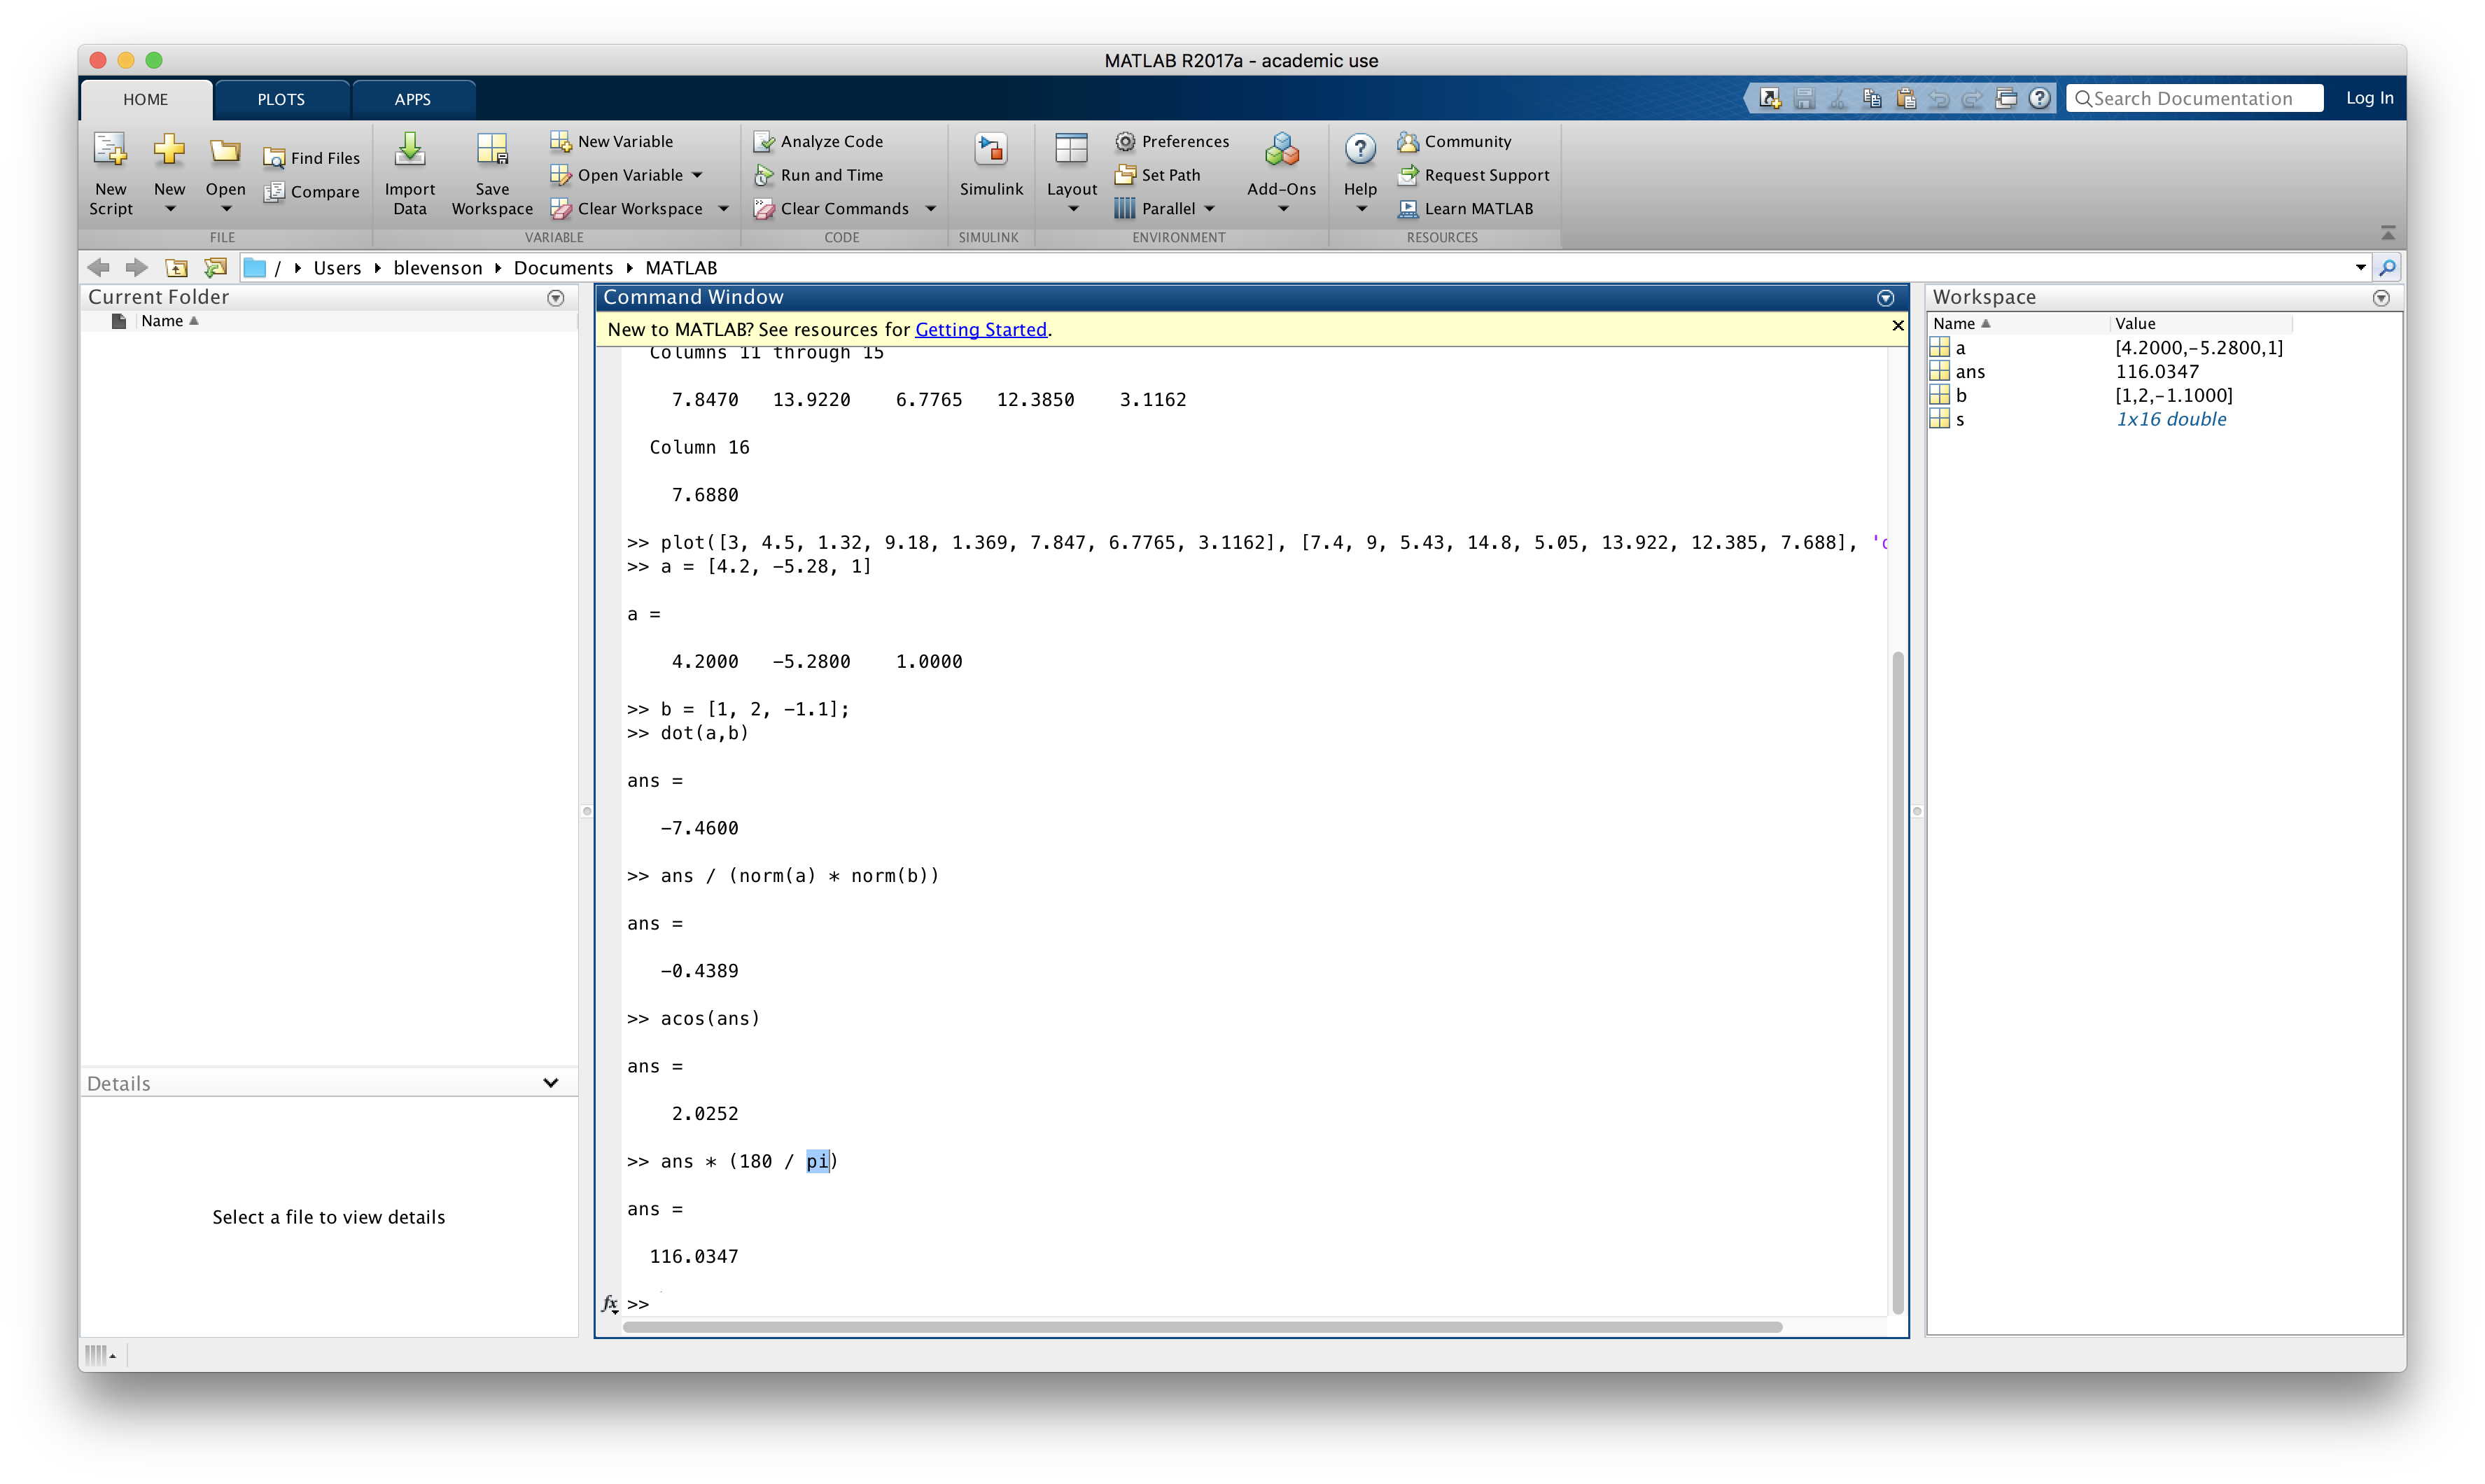
\includegraphics[scale=0.25]{Five}

\end{document}